\documentclass{beamer}
\usepackage[utf8]{inputenc}
\usepackage{graphicx}
\usepackage{listings}
\usepackage{hyperref}
\hypersetup{
	colorlinks=true,
	linkcolor=blue,
	filecolor=magenta,      
	urlcolor=cyan,
}

\urlstyle{same}

\usepackage{xcolor}

\lstdefinestyle{base}{
	language=C++,
	emptylines=1,
	breaklines=true,
	basicstyle=\ttfamily\color{black},
	moredelim=**[is][\bf\color{red}]{@}{@},
}

\usetheme[]{boxes}
\usecolortheme{seagull}
\addtobeamertemplate{navigation symbols}{}{%
	\usebeamerfont{footline}%
	\usebeamercolor[fg]{footline}%
	\hspace{2em}%
	\insertframenumber/\inserttotalframenumber
}

%\usepackage{french}
\title{Modèles et techniques en programmation parallèle hybride et multi-c\oe urs}
\subtitle{Introduction au parall\'elisme multithreads}
\author{Marc Tajchman}\institute{CEA - DEN/DM2S/STMF/LMES}
\date{10/08/2020}

\begin{document}
\begin{frame}
	\titlepage
\end{frame}

\large
\begin{frame}
	\section{Parallélisme multi-threads en mémoire partagée}
	\frametitle{Parallélisme multi-threads en mémoire partagée}

\begin{itemize}
	\item 
	Le but du parallélisme multithreads est de découper l'ensemble des instructions en plusieurs parties et d'exécuter (le plus possible) simultanément ces différentes parties par des threads (exécutions) sur des c\oe urs différents.
	\item 
	On appellera la version du code non parallélisé : ``séquentiel''.
	\item 
    Dans le cas le plus simple, le nombre de threads est égal au nombre de c\oe urs. Mais on peut utiliser un nombre de threads différent du nombre de c\oe urs.
	\item 
	En mémoire partagée signifie que différents groupes d'instructions travaillent sur des données contenues dans la même mémoire. Il faut donc faire attention que les modifications faites par certaines instructions ne perturbent pas les données utilisées par d'autres instructions.
\end{itemize}
\end{frame}

\begin{frame}
	En général, il n'est pas possible de rendre ``multithreads'' la totalité d'un code. Il sera en général composé d'une succession de parties (ou régions) qui devront rester séquentielles et de parties (ou régions) multithreadées.
	\vfill
	
	On aura un enchaînement du type:
	
\begin{minipage}{0.48\textwidth}
	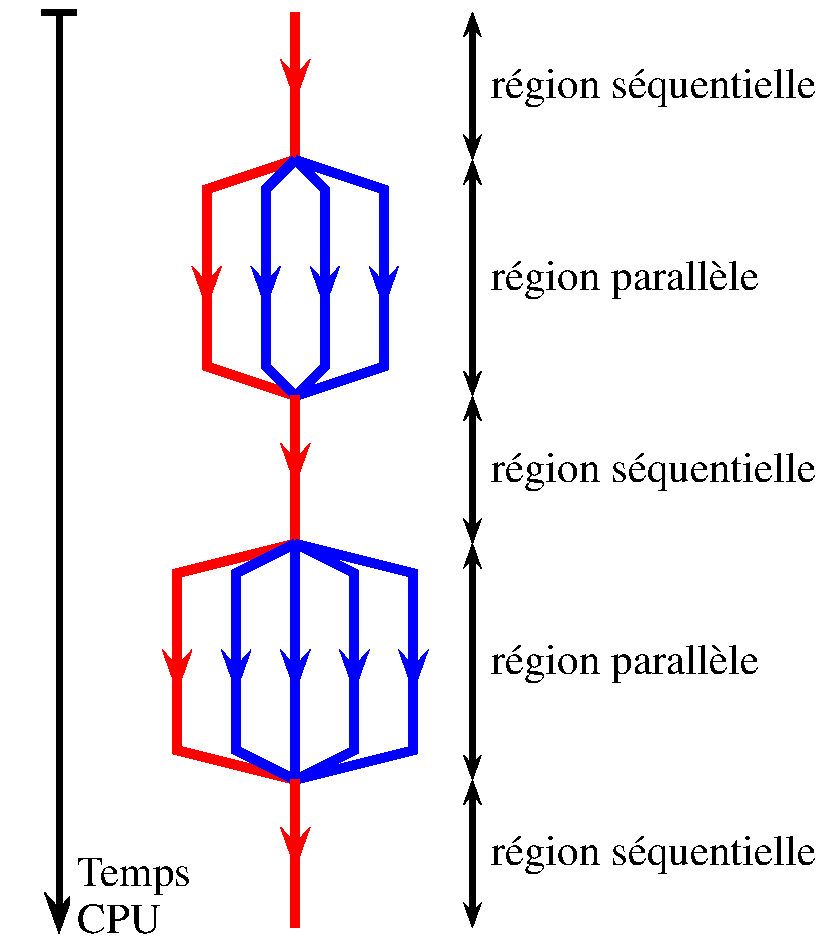
\includegraphics[scale=0.35]{../../Images/enchainement}
\end{minipage}
\begin{minipage}{0.50\textwidth}
	\textcolor{red}{thread${}_0$} : fil d'exécution rouge, actif durant toute l'exécution
	\medskip
	
	\textcolor{blue}{thread${}_i$} ($i > 0$) : un des fils d'exécution bleus, actifs seulement dans des parties parallèles
\end{minipage}
	 
\end{frame}

\begin{frame}[fragile]
	Formellement dans une région parallèle :
	
	\bigskip
	\begin{quote}
On veut exécuter en parallèle, $N$ instructions 
$$
I = \{ I_i(u), i=1 .. N\}
$$ 
où $u$ est une structure de données commune.

\bigskip
On regroupe l'ensemble des instructions en $n_G$ groupes 
$$
G_k = \{ I_{i_j}(u),\quad i_j \in (1..N),\quad j=1,..,N_k\} \quad k = 1 .. n_G
$$

de telle sorte que
$$
\begin{array}{rcl}
G_{k'} \bigcap G_{k''} &=& \varnothing\quad \hbox{ si } k' \neq k'' \\[0.3cm]
\bigcup_{k=1}^{k=n_G} G_k &=& I
\end{array}
$$ 
\end{quote}
	
\end{frame}

\begin{frame}
	
Autrement dit:
\begin{quote}
\textcolor{blue}{Chaque instruction doit être exécutée une et une seule fois} 
\end{quote}

\vfill
\begin{itemize}
	\item Autant que possible, il faut pouvoir exécuter les différents groupes d'instructions de façon indépendante (c'est le système qui décidera de démarrer un groupe, en fonction des c\oe urs disponibles)
	
	\item A l'intérieur d'un groupe, les instructions sont exécutées séquentiellement
	
	\item Il faut déterminer quelles sont les données partagées entre les groupes et celles qui sont privées (utilisées par un seul groupe).  
\end{itemize}

\vfill
Ce dernier point est souvent le plus complexe.
\end{frame}

\begin{frame}[fragile]
Exemple 1:
\vfill
On peut découper une boucle: 
\begin{lstlisting}
for (i=0; i<N; i++)
  v[i] = f(a, u[i]);
\end{lstlisting}

\vfill
en 3 parties (par exemple), \\ \quad avec $0 = N0 \leq N1 \leq N2 \leq N3 = N$:

\vfill
\begin{minipage}{0.52\textwidth}
	\begin{lstlisting}
for (i=N0; i<N1; i++)
  v[i] = f(a, u[i]);
\end{lstlisting}
\end{minipage}
\begin{minipage}{0.46\textwidth}
	$1^{\hbox{er}}$ groupe d'instructions à exécuter par le $1^{\hbox{er}}$ thread
\end{minipage}

%\hline
\begin{minipage}{0.52\textwidth}
\begin{lstlisting}
for (i=N1; i<N2; i++)
  v[i] = f(a, u[i]);
\end{lstlisting}
\end{minipage}
\begin{minipage}{0.46\textwidth}
	$2^{\hbox{ème}}$ groupe d'instructions à exécuter par le $2^{\hbox{ème}}$ thread
\end{minipage}

%\hline
\begin{minipage}{0.52\textwidth}
\begin{lstlisting}
for (i=N2; i<N3; i++)
  v[i] = f(a, u[i]);
\end{lstlisting}
\end{minipage}
\begin{minipage}{0.46\textwidth}
	$3^{\hbox{ème}}$ groupe d'instructions à exécuter par le $3^{\hbox{ème}}$ thread
\end{minipage}

\end{frame}
	
\begin{frame}[fragile]
Il faut examiner l'utilisation de toutes les données sinon on risque de tomber sur des erreurs difficiles à corriger.

\vfill
\begin{tabular}{|l|l|}
	 \hline
	\bf Donnée & \bf Comportement \\
	 \hline
	 \begin{minipage}[t]{0.20\textwidth}
	 	N0, N1, N2, N3, a 
	\end{minipage}
 & \begin{minipage}[t]{0.78\textwidth}
	 	Utilisées par plusieurs threads mais constantes dans l'algorithme, on peut les partager entre les threads
 	\end{minipage}
 	 \\[25pt]
	 \hline
	 u &  \begin{minipage}[t]{0.75\textwidth}
	 	u est constant et donc peut être partagé\end{minipage}
	 \\[10pt]
	 \hline
	 v &  \begin{minipage}[t]{0.75\textwidth}
	 	v varie dans l'algorithme, mais comme chaque thread modifie une partie différente du vecteur, v peut être partagé.\end{minipage}
	 \\[20pt]
	 \hline
	 i &  \begin{minipage}[t]{0.75\textwidth}
	 	i prend des valeurs différentes dans les threads (i = N0 à N1-1 dans le premier thread, i=N1 à N2-1 dans le second thread, etc.), il faut donc utiliser des variables différentes qui représentent i dans les différents threads. i est dit ``variable privée''.\end{minipage}
	 \\[30pt]
	 \hline
\end{tabular}

\end{frame}

\begin{frame}[fragile]
	L'algorithme doit être modifié comme suit:
	
\begin{lstlisting}
for (i0=N0; i0<N1; i0++)
	v[i0] = f(a, u[i0]);
\end{lstlisting}

%\hline
\begin{lstlisting}
for (i1=N1; i1<N2; i1++)
	v[i1] = f(a, u[i1]);
\end{lstlisting}

%\hline
\begin{lstlisting}
for (i2=N2; i2<N3; i2++)
	v[i2] = f(a, u[i2]);
\end{lstlisting}
\vfill

Voir plusieurs variantes dans le répertoire \textcolor{blue}{Exemples2/Exemple1}, codé en OpenMP.

\vfill
Dans le même exemple, on trouvera la façon habituelle (et beaucoup plus simple) de coder une boucle en OpenMP.
\end{frame}

\begin{frame}[fragile]
	Exemple : si \verb|u| et \verb|v| sont des vecteurs de taille \verb|n > 4|, on veut calculer la boucle {\tt for}:

	\begin{equation}
	\begin{array}{l}
for (i=1; i<n-1; i++) \\
\quad  v_i = (u_{i-1} + 2 u_{i} + u_{i+1})/4;
\end{array}
	\end{equation}


	On va examiner en détail le calcul simultané sur 2 c\oe urs des 2 expressions
	
	$$
	\begin{array}{lcl}
	v_2 & = & (u_1 + 2 u_2 + u_3)/4 \\[0.4cm]
	v_3 & = & (u_2 + 2 u_3 + u_4)/4
	\end{array}	
	$$
	
	On supposera que chaque c\oe ur possède sa mémoire cache de taille 8 (4 lignes de cache de taille 2).
\end{frame}

\begin{frame}
	\parbox[t][1cm]{10cm}{1. Avant d'exécuter les 2 instructions :}
   \begin{center}
   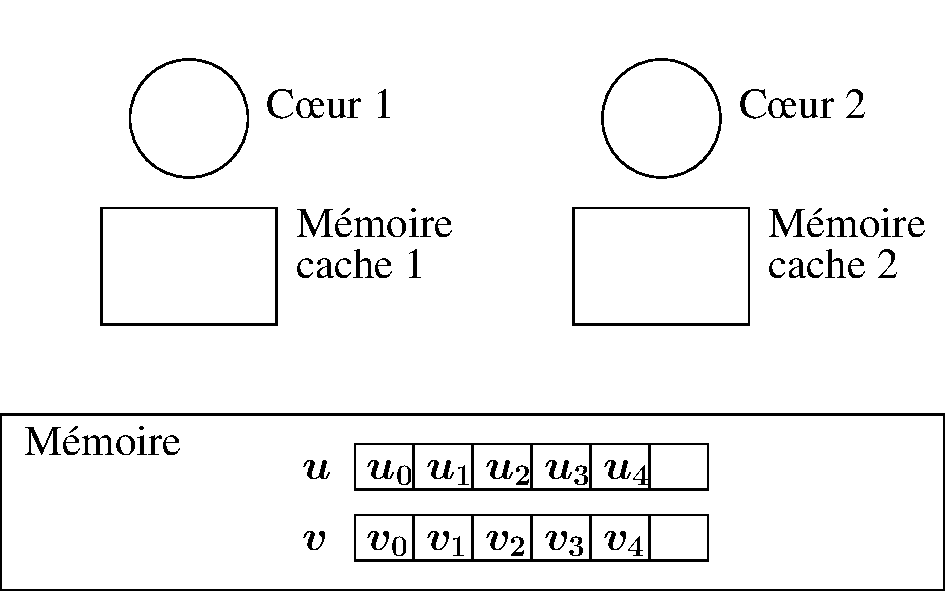
\includegraphics[scale=0.6]{../../Images/multithread0}
   \end{center}
\end{frame}

\begin{frame}
	\parbox[t][1cm]{10cm}{2. Les blocs qui contiennent les composantes utilisées sont recopiés dans les mémoires cache :}
   \begin{center}
	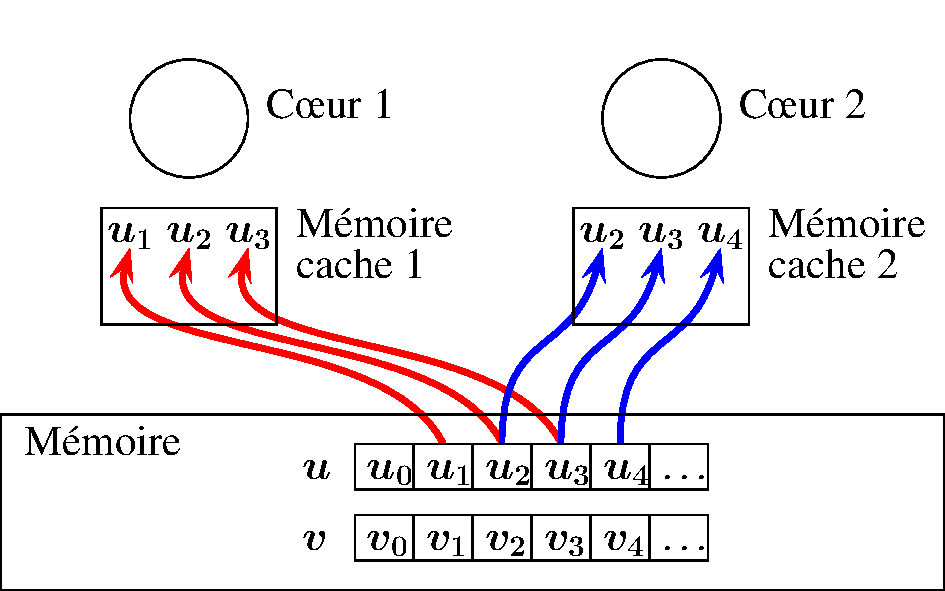
\includegraphics[scale=0.6]{../../Images/multithread1}
   \end{center}
\end{frame}

\begin{frame}
	\parbox[t][1cm]{10cm}{3. Les composantes de $u$ sont recopiées dans les mémoires internes des processeurs et les résultats sont mis à la place de composantes de $v$:} 
	
   \begin{center}
	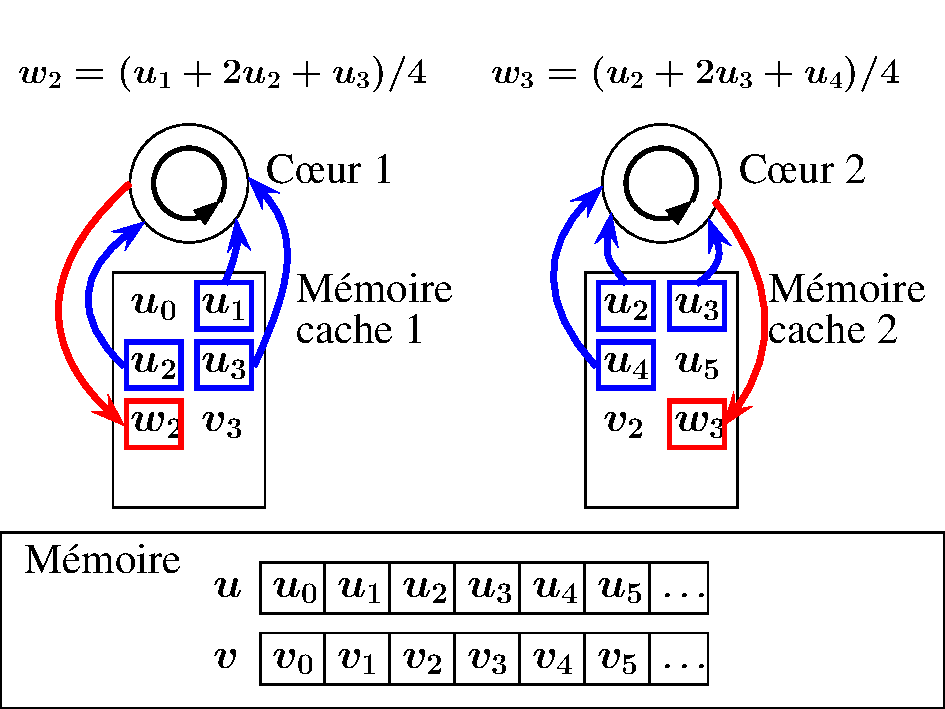
\includegraphics[scale=0.6]{../../Images/multithread2}
   \end{center}
\end{frame}

\begin{frame}
	\parbox[t][1cm]{10cm}{4. Les blocs qui contiennent les résultats sont copiés dans la mémoire centrale. 
\includegraphics[scale=0.015]{../../Images/A14} \textcolor{red}{Le résultat est indéterminé.} 
	}
   \begin{center}
	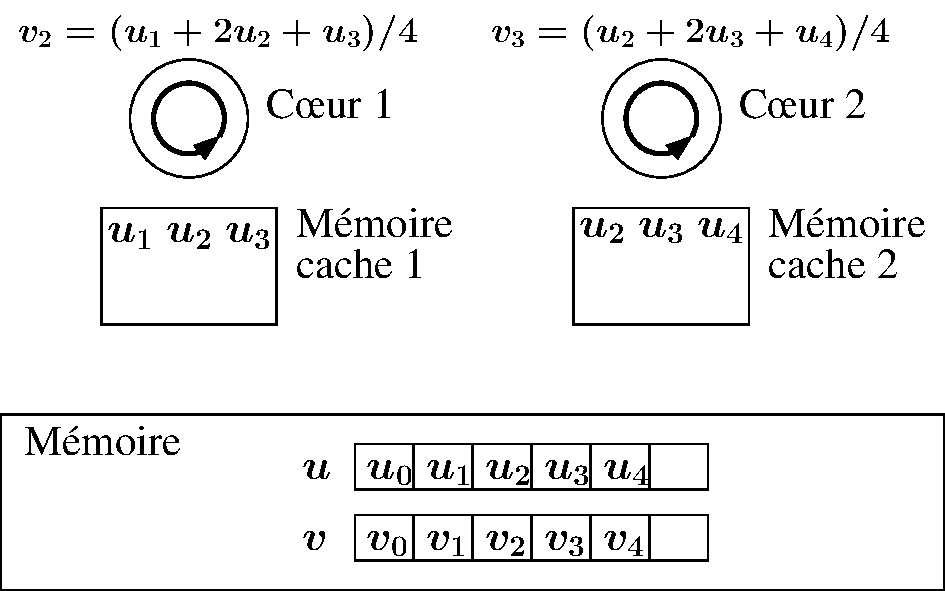
\includegraphics[scale=0.6]{../../Images/multithread3}
   \end{center}
\end{frame}

\begin{frame}
	\vfill
	La collision vient du fait que 2 caches différents contiennent chacun un bloc (partiellement) différent qui sera recopié dans la mémoire centrale au même endroit.
	
	\vfill
	Tous les ordinateurs dont les processeurs ont plusieurs c\oe urs, appliquent un algorithme pour vérifier et rétablir la \textcolor{red}{cohérence de cache} :
	
	\vfill
\begin{quote}
	\textcolor{blue}{Si deux lignes de cache dans deux mémoires cache correspondent au même emplacement dans la mémoire centrale, on garde les valeurs les plus récentes.}
\end{quote}
\vfill

\end{frame}

\begin{frame}
	\parbox[t][1cm]{10cm}{3 bis. On rétablit la cohérence de cache : $w_2$ dans le cache 1 est copié à la place de $v_2$ dans le cache 2 et $w_3$ dans le cache 2 est copié à la place de $v_3$ dans le cache 1}
	\begin{center}
		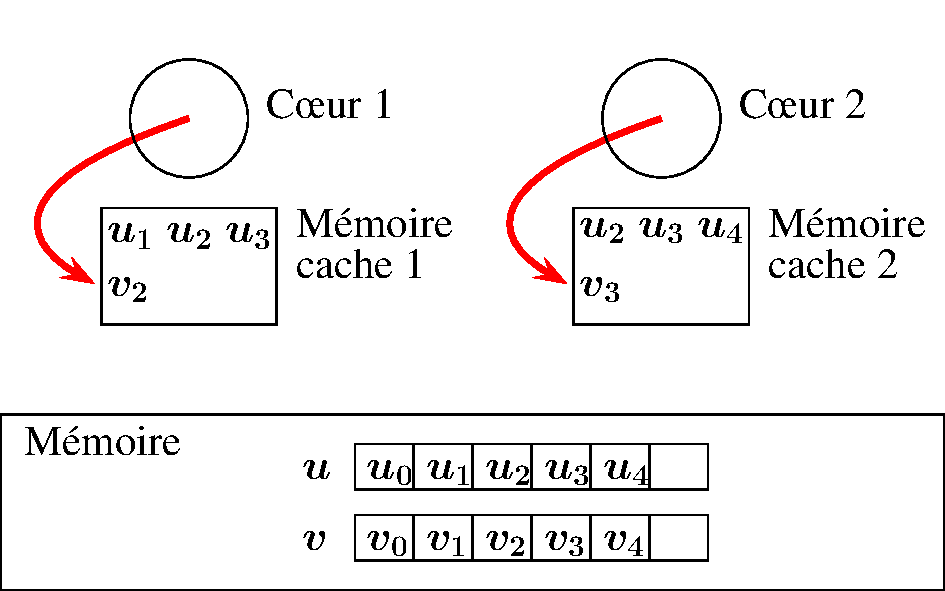
\includegraphics[scale=0.6]{../../Images/multithread4}
	\end{center}
\end{frame}

\begin{frame}
	Grace à l'étape de cohérence de cache les résultats seront corrects mais le maintien de la cohérence de cache prend du temps et diminue l'efficacité du parallélisme multithreads.
	
	\bigskip
	\begin{quote}
		\textcolor{blue}{On essaie de faire en sorte que les caches ne contiennent pas des copies des mêmes blocs mémoires (dans ce cas pas besoin de contrôler la cohérence des caches)}
	\end{quote}
	
\end{frame}

\begin{frame}[fragile]
	D'où la règle supplémentaire :
	\vfill
	
	Règle: 
	\begin{quote}
        \textcolor{red}{Les zones mémoire modifiées par deux threads différents au même instant doivent être distinctes (sinon les résultats peuvent être faux) et assez éloignées (pour diminuer le cout du maintien de la cohérence de cache)}
	\end{quote}
		
	\vfill
	
\end{frame}
\begin{frame}[fragile]
	Exemple: Parcours d'un vecteur $u$ de taille $N$ (multiple de 2) par 2 threads (on suppose que les threads avancent à la même vitesse).
	
\vfill
	Le parcours suivant :
	$$
	\begin{array}{rclrcl}
	\hbox{Thread} 0 & & &\hbox{Thread} 1 & &\\
	u_0 & =& \ldots & u_1 & =& \ldots\\
	u_2 & =& \ldots & u_3 & =& \ldots \\
	u_4 & =& \ldots & u_5 & =& \ldots \\
	... & & ... & \\
	u_{N-2} & = &\ldots & u_{N-1} & = &\ldots \\
	\end{array}
	$$
	est moins bon que le suivant:
$$
\begin{array}{rclrcl}
\hbox{Thread} 0 & & &\hbox{Thread} 1 & &\\
u_0 & =& \ldots & u_{N/2} & =& \ldots\\
u_1 & =& \ldots & u_{N/2+1} & =& \ldots \\
u_2 & =& \ldots & u_{N/2+2} & =& \ldots \\
... & & &... & &\\
u_{N/2-1} & =& \ldots & u_{N-1} & =& \ldots \\
\end{array}
$$
	\vfill
\end{frame}
\begin{frame}
	Dans le premier parcours, les 2 threads travaillent sur des composantes proches $u_k, u_{k+1}$
	\bigskip
	
	Dans le second parcours, les 2 threads travaillent sur des composantes éloignées (on suppose $N$ grand) : $u_k, u_{k+N/2}$
	\vfill
	
	Donc la cohérence de cache sera plus couteuse pour le premier parcours.
	\vfill
\end{frame}

%\begin{frame}[fragile]
%	Le plus simple est de découper la boucle séquentielle :
%
%	\begin{lstlisting}
%for (i=1; i<n-1; i++)
%   v[i] = (u[i-1] + 2*u[i] + u[i+1])/4;
%	\end{lstlisting}
%
%\vfill
%	en $K$ sous-boucles :
%
%\begin{lstlisting}
%for (i=p[k]; i<p[k+1]; i++)    // k = 0...K-1
%   v[i] = (u[i-1] + 2*u[i] + u[i+1])/4;
%\end{lstlisting}
%
%avec {\tt p[0] = 1} et {\tt p[K] = n-1}
%
%\vfill
%L'exécution de toutes les sous-boucles est identique à l'exécution de la boucle complète.
%Toutes les sous-boucles doivent si possible être exécutées en même temps.
%\end{frame}

\begin{frame}[fragile]
	\section{Rappels sur OpenMP}
	\frametitle{Rappels sur OpenMP}
	\vfill
	Le principal (mais pas le seul) outil pour coder du parallélisme multithreads est OpenMP.

    \vfill
    L'exposé ici ne présente que les aspects de base de OpenMP.
    Pour ceux qui veulent réellement utiliser OpenMP dans leurs codes, on conseille l'utilisation de la documentation OpenMP.

\vfill    
    Par exemple:

{\small    
    \begin{quote}
Tim Mattson (Intel) ''Introduction to OpenMP'' 

\url{https://www.openmp.org/wp-content/uploads/Intro_To_OpenMP_Mattson.pdf}

Formation ``OpenMP'' de l'IDRIS (CNRS)

\url{http://www.idris.fr/media/formations/openmp/idris_openmp_cours-v2.10.pdf}

OpenMP API 5.1 Specification 

\url{https://www.openmp.org/wp-content/uploads/OpenMP-API-Specification-5-1.pdf}
\end{quote}
}
     \vfill
\end{frame}

\begin{frame}[fragile]
Principe : on ajoute dans le code, des ``pragma'' (ligne qui commence par \verb|#pragma|)

\vfill
Par exemple:

\vfill
\lstset{%
	language={C++},
	breaklines=true,
	captionpos=b,
	basicstyle=\ttfamily,
	moredelim=[il][\color{red}]{/+},%
}

\begin{lstlisting}{C++}
  /+#pragma omp parallel for

  /+#pragma omp section

  /+#pragma omp critical

  /+#pragma omp master
\end{lstlisting}

\vfill
Si on compile le code sans l'option de compilation OpenMP, les pragmas seront ignorés, donc on peut souvent utiliser le même code source pour un exécutable séquentiel et multithreads.   

\end{frame}

\begin{frame}[fragile]

OpenMP propose aussi quelques fonctions pour gérer le nombre de threads (\verb|omp_get_num_threads()|, \verb|omp_get_num_threads()|) et pour connaître le numéro de thread courant (\verb|omp_get_thread_num()|).

\vfill Ces fonctions ne sont utilisables que dans un code compilé avec OpenMP.

Pour garder un seul code, on peut utiliser la macro {\textunderscore}OPENMP qui vaux vrai si on compile avec OpenMP et faux sinon:
\begin{center}
\lstset{%
	language={C++},
	breaklines=true,
	captionpos=b,
	basicstyle=\ttfamily,
	moredelim=[il][\color{red}]{/+},%
}
\begin{lstlisting}{C++}
/+#ifdef _OPENMP
// code parallele
/+#else
// code sequentiel
/+#endif
\end{lstlisting}
\end{center}

\end{frame}

\begin{frame}

Avantages:
\begin{itemize}
	\item un seul code source pour les versions parallèle ou séquentiel
	\item on peut choisir les boucles qu'on veut paralléliser ou non (parallélisation incrémentale)
	\item facile à coder
\end{itemize}
\vfill

Désavantages et difficultés:
\begin{itemize}
	\item les performances sont parfois décevantes
	\item attention aux variables partagées par différentes itérations d'une boucle
	\item pas beaucoup de contrôle sur le placement des threads et sur le découpage en sous-boucles
\end{itemize}

\end{frame}

\begin{frame}[fragile]

Pour compiler du code utilisant OpenMP, on utilise une option de compilation (qui dépend du compilateur : -fopenmp pour gcc/g++/gfortran).

\vfill
Pour exécuter un code utilisant plusieurs threads, il y a plusieurs possibilités:
\begin{itemize}
	\item définir une variable d'environnement \verb|OMP_NUM_THREADS|, par exemple :
	\begin{lstlisting}
	OMP_NUM_THREADS=5 ./code.exe
	\end{lstlisting}
	\item appeler dans le code source la fonction
	\begin{lstlisting}
	omp_set_num_threads(5);
	\end{lstlisting}
\end{itemize}
\vfill
\end{frame}

\begin{frame}[fragile]
	
	Exemple OpenMP 1
\lstset{%
	language={C++},
	breaklines=true,
	captionpos=b,
	basicstyle=\ttfamily,
	moredelim=[il][\color{red}]{/+},%
}
	\begin{lstlisting}{C++}
/+#pragma omp parallel
{
  std::cout << "Bonjour" << std::endl;
}
\end{lstlisting}

\vfill
{\small
\begin{itemize}
	\item avant d'arriver au pragma, on est dans la partie séquentielle (seul le thread 0 est actif); 
	\item quand l'exécution arrive sur la ligne \verb|#pragma|, le système crée (ou active) $N-1$ threads ($N$ est égal au nombre de c\oe urs ou à la valeur de \verb|OMP_NUM_THREADS| si cette variable d'environnement existe);
	\item chacun des $N$ threads exécute la partie parallèle (le bloc d'instructions contenu entre les accolades);
	\item quand tous les threads sont arrivés à la fin du bloc, les threads s'arrêtent (ou se mettent en pause) sauf le thread 0.
\end{itemize}
}

\end{frame}

\begin{frame}
Le code ci-dessus est contenu dans le répertoire \textcolor{blue}{Exemples2/Exemple\_OpenMP1}.

Lire le fichier README.txt pour compiler et exécuter le code.

\bigskip
Relancer plusieurs fois l'exécution, expliquer ce qui est affiché.

\end{frame}

\begin{frame}[fragile]
	Exemple OpenMP 2 : variables partagées et privées
	\vfill
	
	\lstset{%
	language={C++},
	breaklines=true,
	captionpos=b,
	basicstyle=\ttfamily,
	moredelim=[il][\color{red}]{/+},%
}

\begin{lstlisting}{C++}
std::string prefix = "Ici le thread ";
int iTh;

/+#pragma omp parallel
{
#ifdef _OPENMP
 iTh = omp_get_thread_num();
#else
 iTh = 0;
#endif
 std::cout<<prefix<<iTh<<std::endl;
}
\end{lstlisting}

\vfill
Remarque: la fonction standard \verb|omp_get_thread_num| n'est pas définie si on ne compile pas en mode OpenMP, il faut donc la protéger avec la macro \verb|_OPENMP|
\end{frame}

\begin{frame}[fragile]

	Dans une région parallèle, il faut déterminer la nature des variables:

\begin{itemize}
	\item \verb|prefix| est une chaîne de caractères constante dans la région parallèle, c'est donc une variable partagée entre les threads
	\item \verb|iTh| est un entier qui a une valeur différente dans la région parallèle suivant les threads, c'est donc une variable privée par thread
\end{itemize}

\vfill
Dans la pragma, on liste les variables privées et partagées : 

{\small
\begin{lstlisting}{C++}
#pragma omp parallel shared(v1, v2) private(w1, w2)
\end{lstlisting}
}
\vfill
\textcolor{red}{Si on ne le fait pas, les variables définie dans la région séquentielle et modifiées dans la région parallèle auront une valeur indéterminée}.
\vfill
Souvent les variables sont partagées par défaut, mais on conseille de l'écrire explicitement.
\end{frame}

\begin{frame}[fragile]
	Exemple corrigé:
	
\lstset{%
	language={C++},
	breaklines=true,
	captionpos=b,
	basicstyle=\ttfamily,
	moredelim=[il][\color{red}]{/+},%
}
\begin{lstlisting}{C++}
std::string prefix = "Ici le thread ";
int iTh;

/+#pragma omp parallel shared(prefix) private(iTh)
{
#ifdef _OPENMP
  iTh = omp_get_thread_num();
#else
  iTh = 0;
#endif
  std::cout<< prefix << iTh <<std::endl;
}
\end{lstlisting}

\end{frame}

\begin{frame}[fragile]
	Exemple corrigé (seconde version): on définit \verb|iTh| à l'intérieur de la région parallèle (chaque région parallèle crée sa propre copie de \verb|iTh|) 
	
\lstset{%
		language={C++},
		breaklines=true,
		captionpos=b,
		basicstyle=\ttfamily,
		moredelim=[il][\color{red}]{/+},%
}
\begin{lstlisting}{C++}
std::string prefix = "Ici le thread ";
	
/+#pragma omp parallel shared(prefix)
{
  /+int iTh;
#ifdef _OPENMP
  iTh = omp_get_thread_num();
#else
  iTh = 0;
#endif
  std::cout << prefix << iTh <<std::endl;
}
	\end{lstlisting}
	
\end{frame}

\begin{frame}
	Le code ci-dessus est contenu dans le répertoire \textcolor{blue}{Exemples2/Exemple\_OpenMP2}.
	
	Lire le fichier README.txt pour compiler et exécuter le code.
	
	\bigskip
	Relancer plusieurs fois l'exécution, expliquer ce qui est affiché.
	
\end{frame}

\begin{frame}[fragile]
Exemple OpenMP 3

    \vfill	
    
	Soient $u$, $v$ et $w$ des vecteurs de taille $n$, $a$ et $b$ des scalaires, le code ci-dessous calcule $w = a u + b v$
	\lstset{%
		language={C++},
		breaklines=true,
		captionpos=b,
		basicstyle=\ttfamily,
		moredelim=[il][\color{red}]{/+},%
	}

\vspace{-0.1cm}
\begin{lstlisting}{C++}
  for (i=0; i<n; i++)
    w[i] = a*u[i] + b*v[i];
\end{lstlisting}
\vfill

Pour découper la boucle en T boucles partielles (où T est le nombre de threads), OpenMP propose de le faire lui-même:

\lstset{%
	language={C++},
	breaklines=true,
	captionpos=b,
	basicstyle=\ttfamily,
	moredelim=[il][\color{red}]{/+},%
}

\begin{lstlisting}{C++}
/+#pragma omp parallel \
/+  shared(u,v,w,a,b,n) private(i)
{
/+#pragma omp for
  for (i=0; i<n; i++)
    w[i] = a*u[i] + b*v[i];
}
\end{lstlisting}

\end{frame}

\begin{frame}[fragile]
ou plus simplement:
\lstset{%
	language={C++},
	breaklines=true,
	captionpos=b,
	basicstyle=\ttfamily,
	moredelim=[il][\color{red}]{/+},%
}

\begin{lstlisting}{C++}
/+#pragma omp parallel for \
/+  shared(u,v,w,a,b,n) private(i)
  for (i=0; i<n; i++)
    w[i] = a*u[i] + b*v[i];
\end{lstlisting}

ou encore, si les variables sont partagées par défaut:
\begin{lstlisting}{C++}
/+#pragma omp parallel for
  for (i=0; i<n; i++)
    w[i] = a*u[i] + b*v[i];
\end{lstlisting}

L'indice de boucle qui suit immédiatement le pragma openmp for est implicitement privé
\end{frame}

\begin{frame}
	Le code ci-dessus est contenu dans le répertoire \textcolor{blue}{Exemples2/Exemple\_OpenMP3}.
	
	Lire le fichier README.txt pour compiler et exécuter le code.
		
\end{frame}

\begin{frame}[fragile]
	Exemple OpenMP 4
	
	\vfill	
	
	Soient $A$, $B$ et $C$ des matrices de taille $n\times m$, $a$ et $b$ des scalaires, le code ci-dessous calcule $C = a A + b B$
	\lstset{%
		language={C++},
		breaklines=true,
		captionpos=b,
		basicstyle=\ttfamily,
		moredelim=[il][\color{red}]{/+},%
	}
	
	\vfill

\begin{lstlisting}{C++}
  for (i=0; i<n; i++)
    for (j=0; j<m; j++)
      C(i,j) = a*A(i,j) + b*B(i,j);
\end{lstlisting}
	\vfill
	
	Il y a deux boucles, on a le choix de découper
	\begin{itemize}
		\item la boucle externe sur $i$
		\item la boucle interne sur $j$
		\item les 2 boucles
	\end{itemize}
\end{frame}

\begin{frame}[fragile]
Parallélisation sur la boucle externe :
	\lstset{%
		language={C++},
		breaklines=true,
		captionpos=b,
		basicstyle=\ttfamily,
		moredelim=[il][\color{red}]{/+},%
	}
	
	\begin{lstlisting}{C++}
/+#pragma omp parallel for \
/+    default(shared) private(j)
  for (i=0; i<n; i++)
    for (j=0; j<m; j++)
      C(i,j) = a*A(i,j) + b*B(i,j);
\end{lstlisting}
	\vfill
	Ne pas oublier que seul l'indice $i$ de boucle qui est découpée est implicitement privé.
	\bigskip
	
	L'indice $j$ de la boucle interne doit être privé pour que les résultats soient corrects.
	\vfill
\end{frame}

\begin{frame}[fragile]
	Parallélisation sur la boucle interne :
	\lstset{%
		language={C++},
		breaklines=true,
		captionpos=b,
		basicstyle=\ttfamily,
		moredelim=[il][\color{red}]{/+},%
	}
	
	\begin{lstlisting}{C++}
  for (i=0; i<n; i++)
  {
/+#pragma omp parallel for default(shared)
    for (j=0; j<m; j++)
      C(i,j) = a*A(i,j) + b*B(i,j);
  }
	\end{lstlisting}
	\vfill
	Il y a $n$ régions parallèles (pour chaque itération de la boucle externe).
	
	\vfill
	L'indice de boucle externe $i$ est constant dans les régions parallèles, donc il peut rester partagé.

	\vfill
	L'indice de boucle interne $j$ est implicitement privé.
	\vfill
\end{frame}


\begin{frame}[fragile]
	Parallélisation sur les 2 boucles :
	\lstset{%
		language={C++},
		breaklines=true,
		captionpos=b,
		basicstyle=\ttfamily,
		moredelim=[il][\color{red}]{/+},%
	}
	
	\begin{lstlisting}{C++}
/+#pragma omp parallel for \
/+   default(shared) collapse(2)
for (i=0; i<n; i++)
  for (j=0; j<m; j++)
    C(i,j) = a*A(i,j) + b*B(i,j);
\end{lstlisting}
	\vfill
	Il y a 1 région parallèle.
		
	\vfill
	Les 2 indices de boucle $i$ et $j$ sont implicitement privés.
	\vfill
	Cela ne fonctionne que si les 2 instructions \verb|for| se suivent sans instruction intermédiaire.
\end{frame}

\begin{frame}
	Le code ci-dessus est contenu dans le répertoire \textcolor{blue}{Exemples2/Exemple\_OpenMP4}.
	
	Lire le fichier README.txt pour compiler et exécuter le code.
	
\end{frame}

\begin{frame}
	L'exemple OpenMP 4 suggère les règles suivantes pour améliorer l'efficacité de la parallélisation multithreads:
	
\vfill
	Règle : 
	\begin{quote}
		\textcolor{red}{La quantité d'instructions dans les régions parallèles doit être la plus grande possible par rapport aux instructions dans les régions séquentielles (c'est l'application de la loi d'Amdahl).}
	\end{quote}

\vfill
    Règle :
	\begin{quote}
	\textcolor{red}{Le nombre de régions parallèles doit être le plus petit possible.}
    \end{quote}
\vfill

Règle :
\begin{quote}
	\textcolor{red}{Pour une région parallèle donnée, le nombre de threads qui calcule cette région, doit être déterminé de façon ``optimale''.}
\end{quote}
\vfill
\end{frame}

\begin{frame}
	Le nombre de threads optimal pour calculer une région parallèle est difficile à définir dans l'absolu.
	
\vfill
	Cela dépend du temps mis par le système pour gérer les threads (création, activation, désactivation), pour maintenir la cohérence de cache, etc.
	
\vfill
	Il faut que le temps calcul à l'intérieur du découpage de la région parallèle soit beaucoup plus grand que le temps de gestion multithreads.
	
\vfill
	Cette règle a une signification similaire avec le ratio calculs/communications pour un code MPI.
	
\end{frame}

\begin{frame}
	Dans TBB (une des librairies multithreads) par exemple, la documentation conseille de commencer avec un découpage ou chaque thread passe $\sim 10^5$ cycles dans la région parallèle.
	\bigskip
	
	Le plus raisonnable est de tester : augmenter le nombre de threads (inférieur ou égal au nombre de c\oe urs) tant que la parallélisation améliore le temps calcul.
\vfill
\end{frame}

\begin{frame}[fragile]
	Exemple OpenMP 5
	\vfill
	
	Soit $v$ un vecteur de taille $n$.
	
	\vfill
	On calcule la moyenne et la variance de $v$ par le code suivant
	
	\lstset{%
	language={C++},
	breaklines=true,
	captionpos=b,
	basicstyle=\ttfamily,
	moredelim=[il][\color{red}]{/+},%
}
\begin{lstlisting}{C++}
double s, s2;
for (i=0; i<n; i++) {
  s += v[i];
  s2 += v[i]*v[i];
}
moy = s/n;
var = s2/n - moy*moy;
\end{lstlisting}
	\vfill

Si on divise l'ensemble de itérations en paquets, il faudra faire les sommes de $v_i$ et $v_i^2$ sur chaque paquet puis combiner ces sommes partielles pour obtenir les sommes sur l'ensemble des itérations.	\vfill

\end{frame}

\begin{frame}[fragile]
	Une première version parallélisée serait
	
	\vfill
	\lstset{%
	language={C++},
	breaklines=true,
	captionpos=b,
	basicstyle=\ttfamily,
	moredelim=[il][\color{red}]{/+},%
}
\begin{lstlisting}{C++}
double s, s_partiel[nThreads];
double s2, s2_partiel[nThreads];
int iTh;
/+#pragma omp parallel for \
/+    default(shared) private(iTh)
for (i=0; i<n; i++) {
  iTh = omp_get_thread_num();
  s_partiel[iTh] += v[i];
  s2_partiel[iTh] += v[i]*v[i];
}

s = 0.0; s2 = 0.0;
for (iTh=0; iTh < nThreads; iTh++)
{
  s += s_partiel[iTh];
  s2 += s2_partiel[iTh];
}
moy=s/n; var=s2/n-moy*moy;
\end{lstlisting}
	
\end{frame}

\begin{frame}
	Cette version est très fortement pénalisée par une mauvaise utilisation de la mémoire cache.
	
	On peut introduire un décalage entre les positions mémoires des vecteurs sommes partielles pour améliorer son comportement.
\end{frame}

\begin{frame}[fragile]
	Une seconde version utilise les section critiques OpenMP (ou mieux les sections ``atomiques'')
	
	\vfill
\lstset{%
	language={C++},
	breaklines=true,
	captionpos=b,
	basicstyle=\ttfamily,
	moredelim=[il][\color{red}]{/+},%
}
\begin{lstlisting}{C++}
double s = 0, s_partiel;
double s2 = 0, s2_partiel;

/+#pragma omp parallel default(shared) \
/+      private(s_partiel, s2_partiel) 
{
 s_partiel = 0.0;s2_partiel = 0.0;
/+#pragma omp for
 for (i=0; i<n; i++) {
   s_partiel+=v[i];s2_partiel+=v[i]*v[i];
 }
/+#pragma critical
 {
   s+=s_partiel;s2+=s2_partiel;
 }
}
moy=s/n; var=s2/n-moy*moy;
\end{lstlisting}

	
\end{frame}

\begin{frame}
	Une section critique protège des instructions qui ne peuvent pas être exécutées par plusieurs threads au même moment.
	
	\bigskip
	Quand plusieurs threads arrivent au début de la section critique, ils rentrent dans la section critique l'un après l'autre. 
	
	\bigskip
	Donc une section critique diminue le parallélisme du code mais permet d'éviter des collisions mémoire (plusieurs threads veulent mettre à jour les mêmes variables)
\end{frame}

\begin{frame}[fragile]
Une dernière version utilise le mécanisme de réduction proposé par OpenMP:

\lstset{%
	language={C++},
	breaklines=true,
	captionpos=b,
	basicstyle=\ttfamily,
	moredelim=[il][\color{red}]{/+},%
}
\begin{lstlisting}{C++}
double s = 0 ;
double s2 = 0;

/+# pragma omp parallel for \
/+     default(shared) reduction(+: s, s2)
for (i=0; i<n; i++) {
  s += u[i];
  s2 += u[i]*u[i];
}
moy = s / n ; 
var = s2 /n - moy * moy ;
\end{lstlisting}
\end{frame}

\begin{frame}[fragile]
Quelques autres pragmas

\lstset{%
	language={C++},
	breaklines=true,
	captionpos=b,
	basicstyle=\ttfamily,
	moredelim=[il][\color{red}]{/+},%
}
\begin{lstlisting}{C++}
/+#pragma omp barrier
\end{lstlisting}

\begin{quote}
	Dans une région parallèle, les threads avancent indé\-pen\-dam\-ment les uns des autres. 
	
	Il faut parfois définir des barrières intermédiaires : si certains threads atteignent une position dans le code avant les autres, ils attendent les autres threads.
	
	Les pragma \textcolor{red}{\tt omp parallel} et  \textcolor{red}{\tt omp for} sont suivis d'une barrière implicite.
\end{quote}
\vfill

\end{frame}

\begin{frame}[fragile]

\vfill 
\lstset{%
	language={C++},
	breaklines=true,
	captionpos=b,
	basicstyle=\ttfamily,
	moredelim=[il][\color{red}]{/+},%
}
\begin{lstlisting}{C++}
/+#pragma omp single
\end{lstlisting}

\begin{quote}
	Définit une sous-région dans une région parallèle. Le premier thread qui atteint le début de la sous-région, exécute les instructions qui sont dedans.
	
	Les autres threads sautent au-dessus de cette sous-région.
	
	\textcolor{red}{Il y a une barrière implicite à la fin de la sous-région.}	
\end{quote}
\begin{lstlisting}{C++}
/+#pragma omp master
\end{lstlisting}

\begin{quote}
	Définit une sous-région dans une région parallèle. Seul le thread 0 peut entrer dans la sous-région, et exécuter les instructions qui sont dedans.
	
	Les autres threads sautent au-dessus de cette sous-région.
	
	\textcolor{red}{Il y a pas de barrière implicite à la fin de la sous-région.} 
\end{quote}
\vfill 
\end{frame}
\end{document}
